\documentclass[border=4pt]{standalone}
% Preámbulo común de las figuras. Cada figura es un documento standalone
% que se compila a SVG con scripts/build_figures.sh
\usepackage[utf8]{inputenc}
\usepackage{amsmath}
\usepackage{tikz}
\usepackage[american, siunitx]{circuitikz}
\usetikzlibrary{arrows.meta,calc,decorations.pathmorphing,patterns}
\tikzset{
  >={Stealth[length=2.2mm]},
  eje/.style={->, thin},
  hilo/.style={thick},
}
% Paleta común: tonos medios legibles sobre fondo claro
\definecolor{azul}{RGB}{31,94,168}
\definecolor{rojo}{RGB}{192,57,43}
\definecolor{verde}{RGB}{39,128,73}
\definecolor{naranja}{RGB}{211,120,30}
\definecolor{morado}{RGB}{125,60,152}

\begin{document}
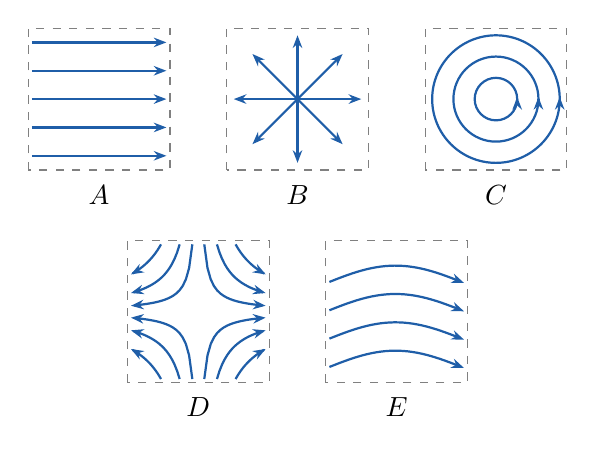
\begin{tikzpicture}[scale=0.9, >={Stealth[length=1.6mm]}]
  \tikzset{caja/.style={dashed, gray}, linea/.style={thick, ->, azul}}
  % A: uniforme
  \begin{scope}[shift={(0,0)}]
    \draw[caja] (0,0) rectangle (2,2);
    \foreach \y in {0.3,0.7,1.1,1.5,1.9} \draw[linea] (0.05,{\y-0.1}) -- (1.95,{\y-0.1});
    \node at (1,-0.35) {$A$};
  \end{scope}
  % B: radial
  \begin{scope}[shift={(2.8,0)}]
    \draw[caja] (0,0) rectangle (2,2);
    \foreach \a in {0,45,...,315} \draw[linea] (1,1) -- ++(\a:0.9);
    \node at (1,-0.35) {$B$};
  \end{scope}
  % C: circular
  \begin{scope}[shift={(5.6,0)}]
    \draw[caja] (0,0) rectangle (2,2);
    \foreach \r in {0.3,0.6,0.9} {
      \draw[thick, azul] (1,1) circle (\r);
      \draw[thick, ->, azul] ({1+\r},1.0) -- ({1+\r},1.03);
    }
    \node at (1,-0.35) {$C$};
  \end{scope}
  % D: silla (hiperbolas)
  \begin{scope}[shift={(1.4,-3)}]
    \draw[caja] (0,0) rectangle (2,2);
    \foreach \c in {0.08,0.25,0.5} {
      \draw[linea] plot[domain={\c/0.95}:0.95, samples=20] ({1+\x},{1+\c/\x});
      \draw[linea] plot[domain={\c/0.95}:0.95, samples=20] ({1+\x},{1-\c/\x});
      \draw[linea] plot[domain={\c/0.95}:0.95, samples=20] ({1-\x},{1+\c/\x});
      \draw[linea] plot[domain={\c/0.95}:0.95, samples=20] ({1-\x},{1-\c/\x});
    }
    \node at (1,-0.35) {$D$};
  \end{scope}
  % E: lineas curvas paralelas
  \begin{scope}[shift={(4.2,-3)}]
    \draw[caja] (0,0) rectangle (2,2);
    \foreach \y in {0.2,0.6,1.0,1.4} \draw[linea] plot[domain=0.05:1.95, samples=30] (\x,{\y + 0.25*sin(deg(\x*1.6))});
    \node at (1,-0.35) {$E$};
  \end{scope}
\end{tikzpicture}
\end{document}
